
\documentclass{beamer}

\usepackage{graphicx,hyperref,udesc,url}
\usepackage[latin1]{inputenc}
%\usepackage[T1]{fontenc}
\usepackage{booktabs}
\usepackage[portuges]{babel}


\title[STGP]{Programa��o Gen�tica Fortemente Tipada\\ com Restri��es Sint�ticas}

\author[Rafael Castro]{
    Rafael Castro\\\medskip
    {\small \url{rafaelcgs10@gmail.com}}}

\date{4 de Dezembro de 2017}

    \institute[UDESC]{
        Departamento de Ci\^encia da Computa\c{c}\~ao \\
            Centro de Ci\^encias e Tecnol\'ogicas\\
            Universidade do Estado de Santa Catarina}

\begin{document}

\begin{frame}
\titlepage

\end{frame}

\section{Introdu��o}
\begin{frame}
\frametitle{O que s�o assistentes de provas?}
\begin{itemize}
    \item Assistentes de provas ou provadores interativos s�o programas para o desenvolvimento de provas
          formais.
    \item Fornecerem informa��es ao programador e verificam a consist�ncia l�gica da prova.\\
          Portanto, erros s�o detectados de maneira imediata.
    \item Provadores autom�ticos fazem todo o trabalho. Assistentes de provas podem utilizar provadores autom�ticos,
          mas ainda necessitam do humano.
\end{itemize}
\end{frame}

\begin{frame}
\frametitle{Para que servem os assistentes de provas?}
\begin{itemize}
        \begin{columns}
            \begin{column}{0.35\textwidth}
            \item Facilitam provar coisas: 
            \end{column}
            \begin{column}{0.41\textwidth}  %%<--- here
        \begin{figure}
            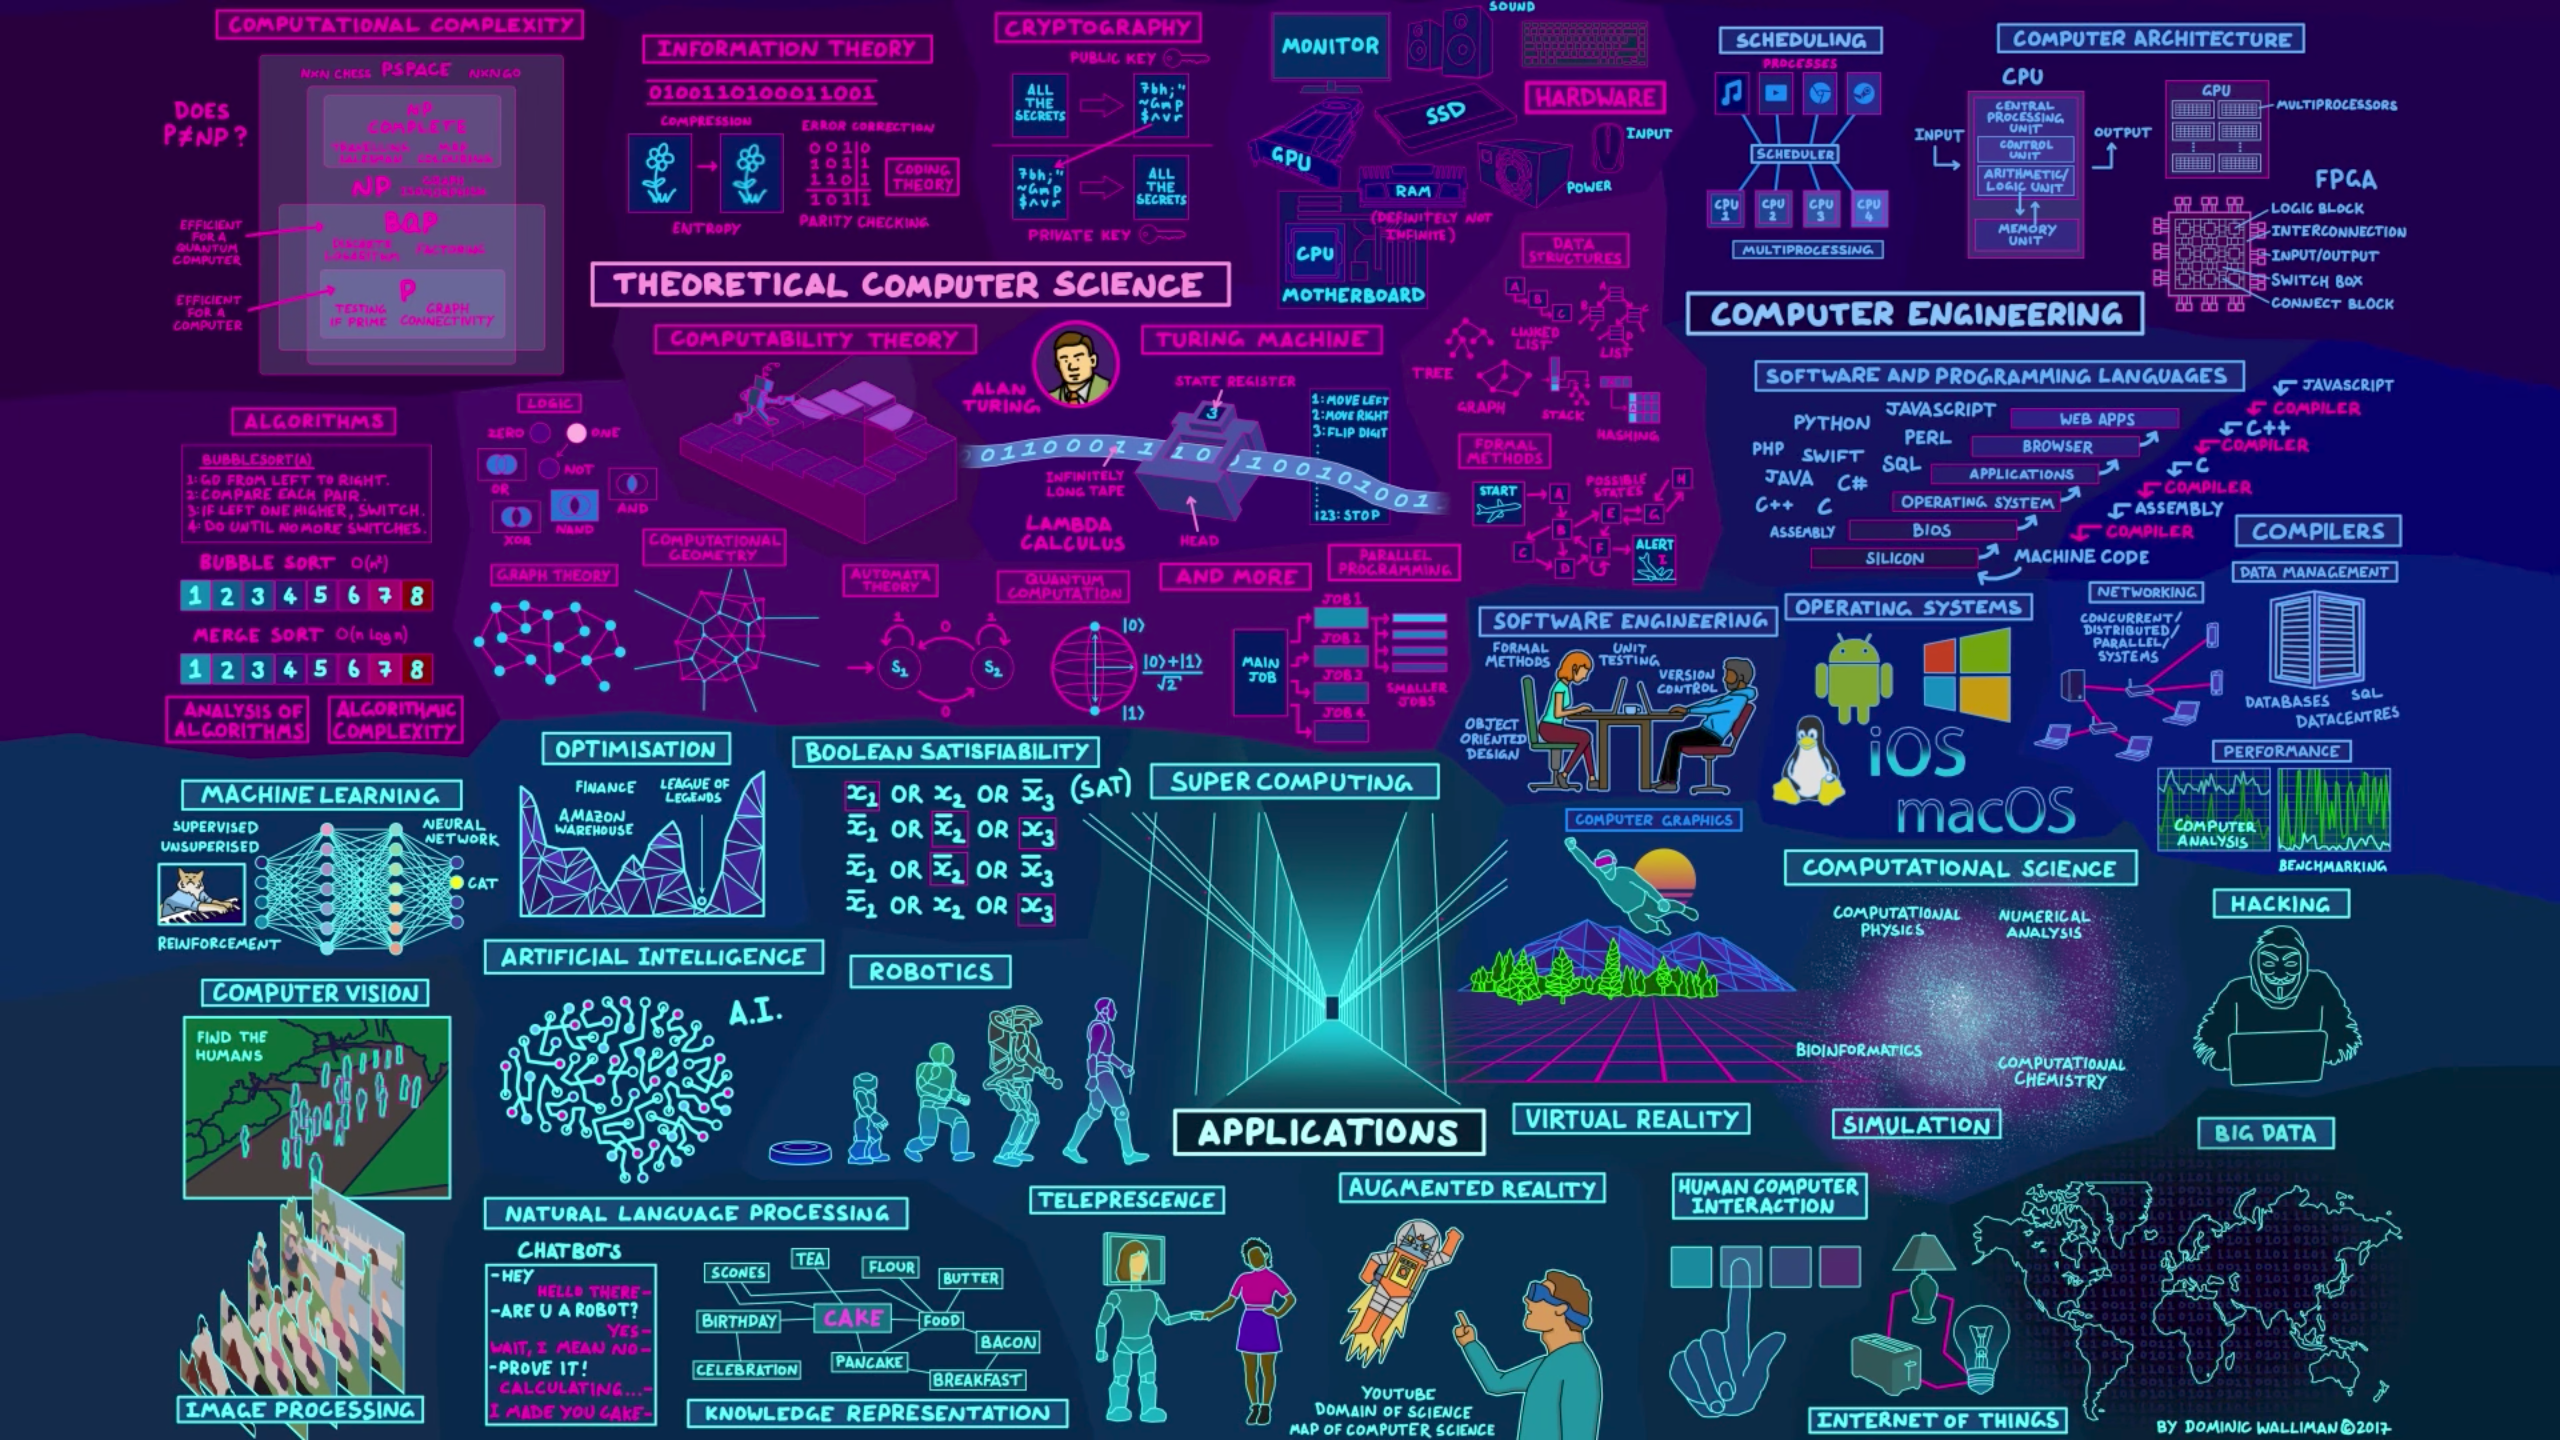
\includegraphics[width=1.0\textwidth]{map.png}
        \end{figure}
            \end{column}
        \end{columns}
    \item A verifica��o autom�tica � �til para evitar o gasto dispendioso de verificar uma prova
          escrita em linguagem humana.
    \item � poss�vel verificar programas. Programa��o certificada.
    \item Uma ferramenta para M�todos Formais.
\end{itemize}
\end{frame}

\section{Coq }
\begin{frame}
\frametitle{O que � Coq?}
\begin{itemize}
    \item Assistente de provas baseado no C�lculo de Constru��es (CoC) - C�lculo Lambda Tipado e Tunado. Estendido para
        C�lculo de Constru��es Indutivas.
    \item L�gica de ordem superior.
    \item Programas verificados (ou provas) em Coq podem ser extra�dos para outras linguagens como Haskell, OCaml e Scheme.
    \item Programa��o com tipos dependentes.
        \begin{enumerate}
            \item Gallina: linguagem de programa\c{c}c\~ao funcional e linguagem de l\'ogica de ordem superior.
            \item Vernecular: linguagem para enunciar teoremas, definir fun\c{c}\~oes ...
            \item Tatic: linguagem para criar provas com a ajuda do assistente/verificador.
        \end{enumerate}
\end{itemize}
\end{frame}

\section{Prova em Coq}
\begin{frame}
\frametitle{Uma prova}
        \begin{figure}
            \centering
            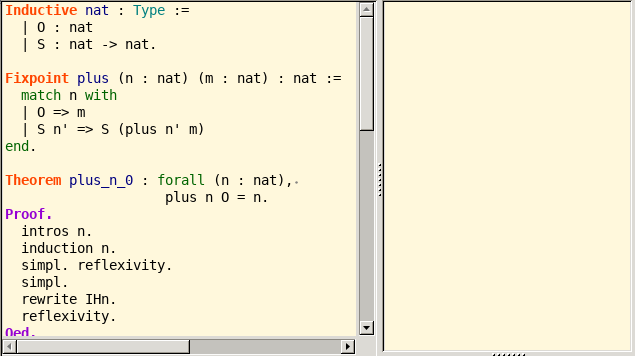
\includegraphics[width=1.05\textwidth]{prova1.png}
        \end{figure}
\end{frame}

\begin{frame}
\frametitle{Uma prova}
\addtocounter{framenumber}{-1}
        \begin{figure}
            \centering
            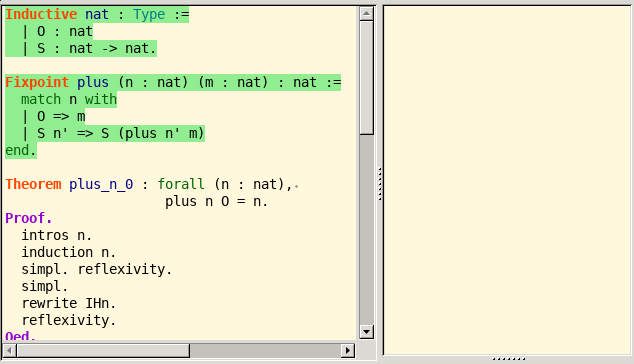
\includegraphics[width=1.05\textwidth]{prova2.png}
        \end{figure}
\end{frame}

\begin{frame}
\frametitle{Uma prova}
\addtocounter{framenumber}{-1}
        \begin{figure}
            \centering
            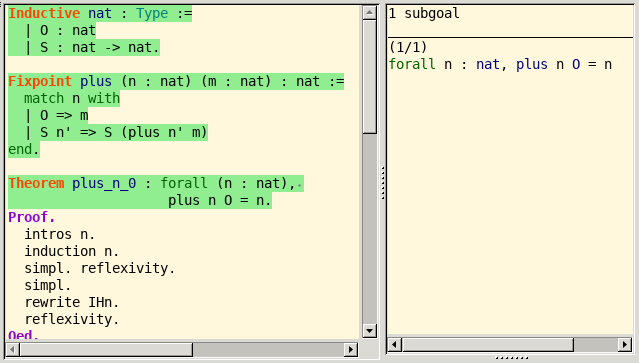
\includegraphics[width=1.05\textwidth]{prova3.png}
        \end{figure}
\end{frame}

\begin{frame}
\frametitle{Uma prova}
\addtocounter{framenumber}{-1}
        \begin{figure}
            \centering
            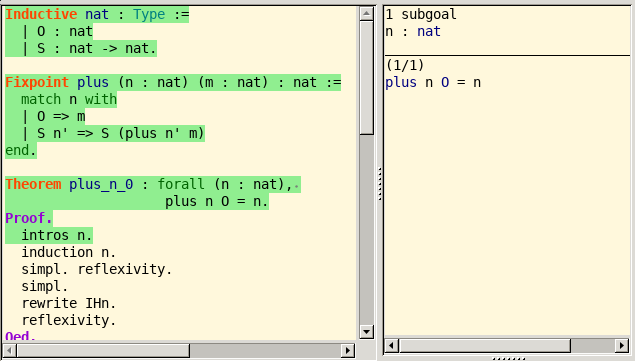
\includegraphics[width=1.05\textwidth]{prova4.png}
        \end{figure}
\end{frame}

\begin{frame}
\frametitle{Uma prova}
\addtocounter{framenumber}{-1}
        \begin{figure}
            \centering
            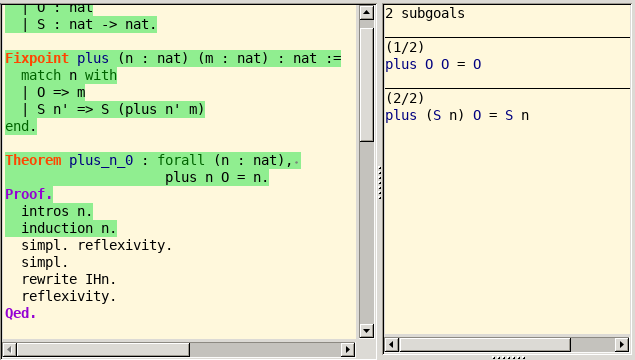
\includegraphics[width=1.05\textwidth]{prova5.png}
        \end{figure}
\end{frame}

\begin{frame}
\frametitle{Uma prova}
\addtocounter{framenumber}{-1}
        \begin{figure}
            \centering
            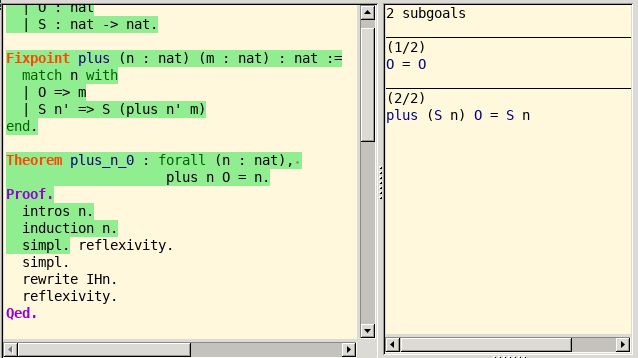
\includegraphics[width=1.05\textwidth]{prova6.png}
        \end{figure}
\end{frame}

\begin{frame}
\frametitle{Uma prova}
\addtocounter{framenumber}{-1}
        \begin{figure}
            \centering
            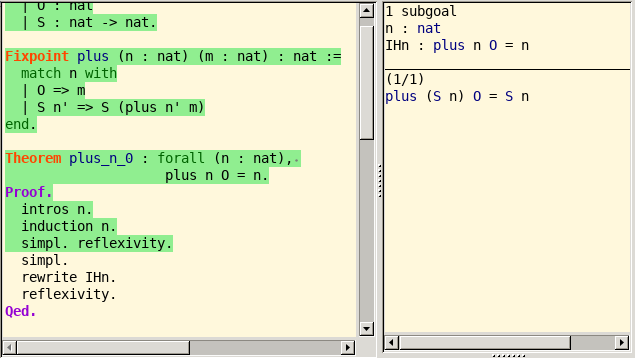
\includegraphics[width=1.05\textwidth]{prova7.png}
        \end{figure}
\end{frame}

\begin{frame}
\frametitle{Uma prova}
\addtocounter{framenumber}{-1}
        \begin{figure}
            \centering
            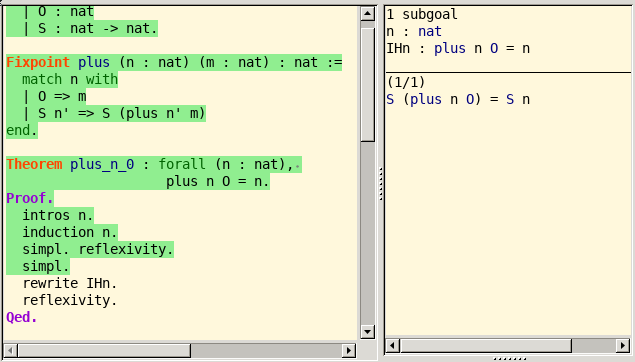
\includegraphics[width=1.05\textwidth]{prova8.png}
        \end{figure}
\end{frame}

\begin{frame}
\frametitle{Uma prova}
\addtocounter{framenumber}{-1}
        \begin{figure}
            \centering
            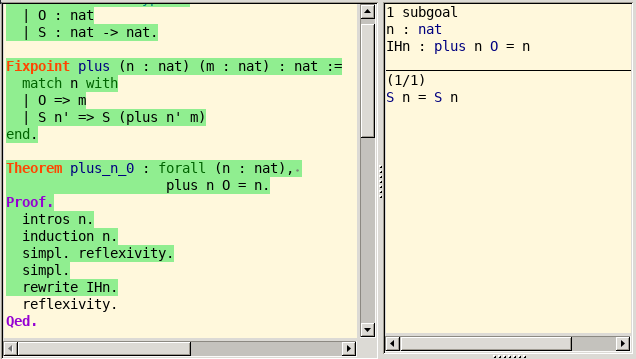
\includegraphics[width=1.05\textwidth]{prova9.png}
        \end{figure}
\end{frame}

\begin{frame}
\frametitle{Uma prova}
\addtocounter{framenumber}{-1}
        \begin{figure}
            \centering
            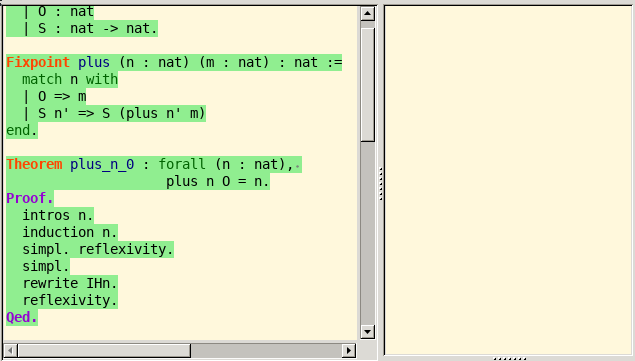
\includegraphics[width=1.05\textwidth]{prova10.png}
        \end{figure}
\end{frame}


\end{document}

